
\pagebreak
\section*{Tydzień 4}
Analiza częstotliwościowa systemów dynamicznych (Transmitancja)\\
\\
\textbf{Transmitancja - $G(s)$}
\begin{figure}[!h]
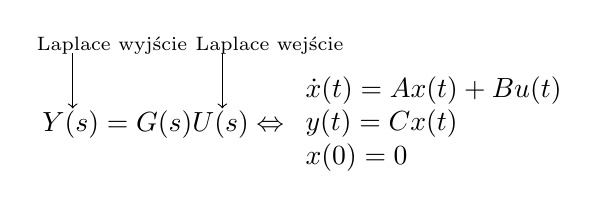
\begin{tikzpicture}
	\node at(0,0) {$Y(s)=G(s)U(s) \Leftrightarrow \begin{array}{l}\dot{x}(t)=Ax(t)+Bu(t)\\y(t)=Cx(t)\\x(0)=0\end{array}$};
	\node at(-2.5,1)[font=\scriptsize]{Laplace wyjście};
	\node at(-0.5,1)[font=\scriptsize]{Laplace wejście};
	\draw[->](-3,.9)--(-3,0.2);
	\draw[->](-1.1,.9)--(-1.1,0.2);
\end{tikzpicture}
\end{figure}
\\
$G(s)=C(sI-A)^{-1}B$\\
\\
\fbox{\parbox{.6\linewidth}{
	\textbf{Kryterium Michajłowa}\\
	$G(s)=\frac{L(s)}{M(s)}$\\
	$M(s)=a_ns^n+a_{n-1}s^{n-1}+...+a_1s+a_0$\\
	Układ jest asymptotycznie stabilny jeśli przyrost argumentu $M(j\omega)$ rzędu $n$ przy zmianie $\omega$ od $-\infty$ do $+\infty$ wynosi $n\pi$: $\Delta Arg \ M(j\omega)|^{+\infty}_{-\infty}=n\pi$\\
}}\\\\
\fbox{\parbox{.6\linewidth}{
	\textbf{Kryterium Nyquista}\\
	Jeżeli układ otwarty opisany transmitancją $G(s)$ jest asymptotycznie stabilny, to układ ze sprzężeniem zwrotnym, opisany za pomocą transmitancji $G_z(s)$ jest asymptotycznie stabilny wtedy i tylko wtedy, gdy wykres charakterystyki amplitudowo-fazowej transmitancji $G(s)$ nie obejmuje punktu $(-1,0)$ na płaszczyźnie zespolonej.
}}\\\\
\\
Laplace :\\
$e^{ax} \leftrightarrow \frac1{s-a}$\\
$1 \leftrightarrow \frac1s$\\

\pagebreak
%###################                 4.1.1              #################################%
\subsection*{Zadanie 4.1.1} {\color{darkgray}
	Układ jest opisany równaniami stanu w postaci\\\\
	$\begin{cases} \dot{x}(t)=Ax(t)+Bu(t)\\y(t)=Cx(t)\end{cases}$\\\\
	z macierzami\\\\
	$A=\left[\begin{array}{cc}1&0\\2&-3\end{array}\right],
	B=\left[\begin{array}{c}1\\0\end{array}\right],
	C=\left[\begin{array}{cc}	1&0\end{array}\right]
	$\\\\
	Znaleźć transmitancję operatorową tego układu przy założeniu zerowych warunków początkowych $x(0)=0$\\
}\lineh
\\\\
$G(s)=C(sI-A)^{-1} \cdot B$\\
$(sI-A)^{-1}=\left[\begin{array}{cc}s-1&0\\-2&s-3\end{array}\right]^{-1}=\frac{1}{(s-1)(s-3)}\left[\begin{array}{cc}s-3&0\\2&s-1\end{array}\right]=\left[\begin{array}{cc}\frac{1}{s-1}&0\\\frac{2}{(s-1)(s-3)}&\frac{1}{s-3}\end{array}\right]$\\
$G(s)=\left[\begin{array}{cc}1&0\end{array}\right]\cdot\left[\begin{array}{cc}\frac{1}{s-1}&0\\\frac{2}{(s-1)(s-3)}&\frac{1}{s-3}\end{array}\right]\cdot \left[\begin{array}{c}1\\0\end{array}\right]=\left[\begin{array}{cc}\frac{1}{s-1}&0\end{array}\right] \cdot \left[\begin{array}{c}1\\0\end{array}\right]=\frac{1}{s-1}$\\



%###################                 4.1.2              #################################%
\pagebreak
\subsection*{Zadanie 4.1.2} {\color{darkgray}
	Układ jest opisany równaniami stanu w postaci\\\\
	$\begin{cases} \dot{x}(t)=Ax(t)+Bu(t)\\y(t)=Cx(t)\end{cases}$\\\\
	z macierzami\\\\
	$A=\left[\begin{array}{cc}2&0\\-5&0\end{array}\right],
	B=\left[\begin{array}{c}2\\2\end{array}\right],
	C=\left[\begin{array}{cc}0&1\end{array}\right]$\\\\
	Znaleźć transmitancję operatorową tego układu przy założeniu zerowych warunków początkowych $x(0)=0$\\
}\lineh
\\\\
$G(s)=C(sI-A)^{-1}B$\\
$G(s)=\left[\begin{array}{cc}0&1\end{array}\right]
\cdot
\left[\begin{array}{cc}{s-2}&0\\5&s\end{array}\right]^{-1}
\cdot
\left[\begin{array}{c}2\\2\end{array}\right]=\left[\begin{array}{cc}0&1\end{array}\right]
\cdot 
\left[\begin{array}{cc}{\frac{1}{s-2}}&0\\\frac{-5}{s(s-2)}&\frac{1}{s}\end{array}\right]
\cdot
\left[\begin{array}{c}2\\2\end{array}\right]=\frac{2}{s}-\frac{10}{s\cdot(s-2)}=\frac{2s-14}{s\dot{(s-2)}}
$

%###################                 4.1.3              #################################%
\pagebreak
\subsection*{Zadanie 4.1.3} 
	Układ jest opisany równaniami stanu w postaci\\\\
\begin{gather*}
\begin{cases}
\dot{x}(t) = \mathbf{A}x(t) + \mathbf{B}u(t) \\
y(t) = \mathbf{C}x(t)
\end{cases}
\\
\mathbf{A} = \begin{bmatrix} 2 & -1 \\ 2 & -5 \end{bmatrix},
\mathbf{B} = \begin{bmatrix} 2 \\ 2 \end{bmatrix},
\mathbf{C} = \begin{bmatrix} 0 & 1 \end{bmatrix}
\end{gather*}

Znaleźć transmitancję operatorową tego układu przy założeniu zerowych warunków początkowych $x(0)=0$\\
\lineh	

Dla $x(0) = 0$ mamy:
\[ G(s) = \mathbf{C} (s\mathbf{I} - \mathbf{A})^{-1} \mathbf{B} \]

\begin{align*}
G(s) & = \mathbf{C} \left(\begin{bmatrix} s & 0 \\ 0 & s \end{bmatrix} - \begin{bmatrix} 2 & -1 \\ 2 & -5 \end{bmatrix}\right)^{-1} \mathbf{B}=\\
& = \mathbf{C} \left(\begin{bmatrix} s-2 & 1 \\ -2 & s+5 \end{bmatrix}\right)^{-1} \mathbf{B} = \\
& = \mathbf{C} \left(\frac{1}{(s+5)(s-2)+2}\right) \begin{bmatrix} s+5 & 2 \\ -1 & s-2 \end{bmatrix}^\mathrm{T} \mathbf{B} = \\
& = \left(\frac{1}{s^2+3s-8}\right) \mathbf{C} \begin{bmatrix} s+5 & -1 \\ 2 & s-2 \end{bmatrix} \mathbf{B} = \\
& = \left(\frac{1}{s^2+3s-8}\right) \begin{bmatrix} 0 & 1 \end{bmatrix}\begin{bmatrix} s+5 & -1 \\ 2 & s-2 \end{bmatrix} \mathbf{B} = \\
& = \left(\frac{1}{s^2+3s-8}\right) \begin{bmatrix} 2 & s-2 \end{bmatrix}\begin{bmatrix} 2 \\ 2 \end{bmatrix} = \\
& = \left(\frac{1}{s^2+3s-8}\right) (4+2s-4) = \frac{2s}{s^2+3s-8}
\end{align*}

Odp: $G(s) = \frac{2s}{s^2+3s-8}$.

%###################                 4.1.3              #################################%
%\pagebreak
%\subsection*{Zadanie 4.1.3} {\color{darkgray}
%	Układ jest opisany równaniami stanu w postaci\\\\
%	$\begin{cases} \dot{x}(t)=Ax(t)+Bu(t)\\y(t)=Cx(t)\end{cases}$\\\\
%	z macierzami\\\\
%	$A=\left[\begin{array}{cc}2&3\\1&0\end{array}\right],
%	B=\left[\begin{array}{c}2\\5\end{array}\right],
%	C=\left[\begin{array}{cc}0&1\end{array}\right]$\\\\
%	Znaleźć transmitancję operatorową tego układu przy założeniu zerowych warunków początkowych $x(0)=0$\\
%}\lineh
%\\\\


%###################                 4.2.1              #################################%
\pagebreak
\subsection*{Zadanie 4.2.1} {\color{darkgray}
	Mając dana transmitancje $G(s)=\frac{5}{s+3}$ określić amplitudę sygnału wyjściowego, jesli na wejście podano:\\
	a) $2\sin(4t+2 \pi)$\\
	b) $-\sin(t)$\\
	c) $0.1\cos(4t+\frac\pi 6)$\\
}\lineh
\\\\
$G(s)=\frac{5}{s+3}$\\
$A(\omega)=|G(j\omega)|$\\
$u(t)=A_u\sin(\omega t+\varphi_u )$ - wejście\\
$A_y=A(\omega) \cdot A_u$\\
\\
\textbf{a)}\\
$2\sin(4t+2\pi)=u(t)$\\
$A_u=2$\\
$\omega=4$\\
$A(\omega)=|\frac{5}{4j+3}|=|\frac{5(3-4j)}{9+16}|=|\frac{3-4j}{5}|=\sqrt{\frac{9}{25}+\frac{16}{25}}=1$\\
$A_y=1 \cdot 2 = \boxed{2}$ \ \ \ \ \ \   {\color{lightgray}$A(\omega)=\frac{5}{\sqrt{16+9}}=1$}\\
\\
\textbf{b)}\\
$-\sin(t)=u(t)$\\
$A_u=-1$\\
$\omega=1$\\
$A(\omega)=|\frac{5}{j+3}|=|\frac{5(3-j)}{9+1}|=|\frac{3-j}{2}|=\sqrt{\frac 94+\frac 14}=\frac{\sqrt{10}}{2}$\\
$A_y=-1 \cdot \frac{\sqrt{10}}{2}=\boxed{-\frac{\sqrt{10}}{2}}$\ \ \ \ \ \ \   {\color{lightgray}$A(\omega)=\frac{5}{\sqrt{9+1}}=\frac{\sqrt{10}}{2}$}\\
\\
\textbf{c)}\\
$0.1\cos(4t+\frac\pi 6)=u(t)$\\
$\cos(\frac\pi 2 - \alpha)=\sin \alpha \Rightarrow \cos(4t+\frac \pi 6 ) = \cos (\frac \pi 2 -(\frac{2\pi}{6} - 4t))= \sin(\frac{2\pi}{6}-4t)$\\
$u(t)=\frac{1}{10}\sin(\frac \pi 3 - 4t)$\\
$A_u = \frac{1}{10} \ \ \ \ \ \omega=-4$\\
$A(\omega)=|\frac{5}{-4j+3}|=|\frac{5(3+4j)}{9+16}|=|\frac{3+4j}{5}|=\sqrt{\frac{9}{25}+\frac{16}{25}}=1$\\
$A_y=1 \cdot \frac{1}{10} = \boxed{\frac{1}{10}}$ \ \ \ \ \ \   {\color{lightgray}$A(\omega)=\frac{5}{\sqrt{16+9}}=1$}\\

%###################                 4.2.2              #################################%
\pagebreak
\subsection*{Zadanie 4.2.2} {\color{darkgray}
	Mając dana transmitancje $G(s)=\frac{1}{s+2}$ okreslić amplitudę sygnału wyjściowego, jesli na wejście podano:\\
	a) $5\sin(2t+ \pi)$\\
	b) $-2\sin(3t)$\\
	c) $0.1\cos(t+\frac\pi 3)$\\
}\lineh
\\\\
$G(s)=\frac{1}{s+2}$\\
$A(\omega)=|G(j\omega)|$\\
$u(t)=A_u\sin(\omega t+\varphi_u )$ - wejście\\
$A_y=A(\omega) \cdot A_u$\\
alternatywnie (nie skonczone)\\
{\color{lightgray}
$A(\omega)=|\frac1{j\omega+2}|=|\frac{j\omega-2}{-\omega^2-4}|=|\frac2{\omega^2+4}+j(\frac{\omega}{-\omega^2-4})|=\sqrt{\frac{4}{(\omega^2+4)^2}-\frac{\omega^2}{(\omega^2+4)^2}}=\sqrt{\frac{(4-\omega)^2}{(\omega^2+4)^2}}=\frac{\sqrt{(2-\omega)(2+\omega)}}{\omega^2+4}$\\
\\
\textbf{a)}\\
$A_y=\frac{\sqrt{(2-\omega)(2+\omega)}}{\omega^2+4} \cdot 5$\\
\textbf{b)}\\
$A_y=\frac{\sqrt{(2-\omega)(2+\omega)}}{\omega^2+4} \cdot (-2)$\\
\textbf{c)}\\
$A_y=\frac{\sqrt{(2-\omega)(2+\omega)}}{\omega^2+4} \cdot (0.1)$\\
}


%###################                 4.2.3              #################################%
\pagebreak
\subsection*{Zadanie 4.2.3} {\color{darkgray}
	Mając dana transmitancje $G(s)=\frac{30}{s+2}$ określić amplitudę sygnału wyjściowego, jeśli na wejście podano:\\
}\lineh
\\\\
\begin{gather*}
u(t) = A_u \cdot \sin{(\omega t+\phi_u)}\text{ - wejście} \\
A_u \text{ - amplituda wejścia} \\
\phi_u \text{ - faza wejścia} \\
y(t) = A_y \cdot \sin{(\omega t+\phi_y)}\text{ - wyjście} \\
A_y = A(\omega) \cdot A_u \text{ - amplituda wyjścia} \\
\phi_y \text{ - faza wyjścia} \\
A(\omega) = |G(j\omega)| \\
G(s) = \frac{300}{s+30}
\end{gather*}

a)
\begin{align*}
u(t) &= -2\sin{(5t)} \\
A_u &= -2 \\
\omega &= 5 \\
A(\omega) &= A(5) = |G(5j)| = \left| \frac{300}{5j+30} \right| 
= \left| \frac{60}{6+j} \cdot \frac{6-j}{6-j} \right|
= \left| \frac{60}{37} \cdot (6-j) \right| = \\
&= \frac{60}{37} \cdot |6-j| = \frac{60}{37} \cdot \sqrt{6^2+(-1)^2} 
= \frac{60 \cdot \sqrt{37}}{37} \\
A_y &= A(\omega) \cdot A_u = \frac{60 \cdot \sqrt{37}}{37} \cdot -2
= \boxed{ \frac{-120 \cdot \sqrt{37}}{37} }
\end{align*}

b)
\begin{align*}
u(t) &= 5\sin{\left( 2t+\frac{\pi}{2} \right)} \\
A_u &= 5 \\
\omega &= 2 \\
A(\omega) &= A(2) = |G(2j)| = \left| \frac{300}{2j+30} \right| 
= \left| \frac{150}{15+j} \cdot \frac{15-j}{15-j} \right|
= \left| \frac{150}{256} \cdot (15-j) \right| = \\
&= \frac{75}{128} \cdot |15-j| = \frac{75}{128} \cdot \sqrt{15^2+(-1)^2} 
= \frac{75 \cdot 16}{128} = \frac{75}{8} \\
A_y &= A(\omega) \cdot A_u = \frac{75}{8} \cdot 5
= \boxed{ \frac{375}{8} }
\end{align*}

c)
\begin{align*}
u(t) &= \cos{\left( 3t+\frac{\pi}{3} \right)} = \sin{\left( 3t+\frac{\pi}{3}+\frac{\pi}{2} \right)}
= \sin{\left( 3t+\frac{5\pi}{6} \right)} \\
A_u &= 1 \\
\omega &= 3 \\
A(\omega) &= A(3) = |G(3j)| = \left| \frac{300}{3j+30} \right| 
= \left| \frac{100}{10+j} \cdot \frac{10-j}{10-j} \right|
= \left| \frac{100}{101} \cdot (10-j) \right| = \\
&= \frac{100}{101} \cdot |10-j| = \frac{100}{101} \cdot \sqrt{10^2+(-1)^2} 
= \frac{100 \cdot \sqrt{101}}{101} \\
A_y &= A(\omega) \cdot A_u = \frac{100 \cdot \sqrt{101}}{101} \cdot 1
= \boxed{ \frac{100 \cdot \sqrt{101}}{101} }
\end{align*}


%###################                 4.3.1              #################################%
\pagebreak
\subsection*{Zadanie 4.3.1} {\color{darkgray}
	Za pomocą transmitancji znaleźć odpowiedź układu 1 na skok jednostkowy, czyli funkcję postaci:\\
	$u(t)=\begin{cases}0,t<0 \\ 1, t\geqslant 0 \end{cases}$\\
	Zakladamy, że $x(0)=0$\\
	$\dot{x}(t)=-4x(t)+8u(t)$\\
	$y(t)=x(t)$\\
}\lineh
\\\\
$C=1 \ \ \ A=-4 \ \ \ \ B=8$\\
$G(s)=1 \cdot (s+4)^{-1} \cdot 8 = 8 \cdot \frac{1}{s+4}$\\
$U(s)=\frac 1 s \ \ \ $\\ tw. Laplace'a dla skoku jednostkowego
$Y(s)=G(s) \cdot U(s)$\\
$Y(s)=\frac{8}{s+4} \cdot \frac{1}{s} = \frac{2}{s} - \frac{2}{s+4}$\\
$\frac{A}{s}+\frac{B}{s+4}=\frac{8}{s(s+4)}$\\
$A(s+4)+Bs=8$\\
$s(A+B)+4A=8$\\
$A=2 \ \ \ B=-2$\\
$\boxed{y(t)=-2e^{-4t}+2}$\\ 
$\uparrow$\\
odwrotne tw. Laplace'a\\
$\mathcal{L}\{a\}=a\frac 1 s$\\
$\mathcal{L}\{ae^{bt}\}=a\frac {1}{s-b}$\\

%###################                 4.3.2              #################################%
\pagebreak
\subsection*{Zadanie 4.3.2} {\color{darkgray}
	Za pomocą transmitancji znaleźć odpowiedź układu 1 na skok jednostkowy, czyli funkcję postaci:\\
	$u(t)=\begin{cases}0,t<0 \\ 1, t\geqslant 0 \end{cases}$\\
	Zakładamy, że $x(0)=0$\\
	
	$
\begin{cases}
\dot{x}(t) = -2x(t) + u(t) \\
y(t) = x(t)
\end{cases}$ \\
}\lineh
%\\\\
\begin{gather*}
u(t) = \begin{cases}
0 & \text{dla } t < 0 \\
1 & \text{dla } t \geqslant  0
\end{cases} \\
\begin{cases}
\dot{x}(t) = -2x(t) + u(t) \\
y(t) = x(t)
\end{cases} \\
\mathbf{A} = -2, \mathbf{B} = 1, \mathbf{C} = 1
\end{gather*}

Dla $x(0) = 0$ mamy:
\[ G(s) = \mathbf{C} (s\mathbf{I} - \mathbf{A})^{-1} \mathbf{B} \]

\begin{equation*}
\begin{aligned}
& G(s) = 1 \cdot [s - (-2)]^{-1} \cdot 1 = \frac{1}{s+2} \\
& U(s) = \mathscr{L}\{u(t)\} = \frac{1}{s} \\
& Y(s) = G(s) \cdot U(s) = \frac{1}{s+2} \cdot \frac{1}{s} \\
& \frac{1}{(s+2)s} = \left. \frac{A}{s+2} + \frac{B}{s} \right| \cdot (s+2)s \\
& 1 = A \cdot s + B \cdot s + 2B = s(A+B) + 2B \\
& \begin{cases}
A+B = 0 \\
2B = 1
\end{cases} \\
& \begin{cases}
B = \frac12 \\
A = -\frac12
\end{cases} \\
& Y(s) = \frac{-\frac12}{s+2} + \frac{\frac12}{s} \\
& y(t) = \mathscr{L}^{-1}\{Y(s)\}
& \begin{array}{rl}
	& \mathscr{L}^{-1}\{\frac{a}{s}\} = a \\
	& \mathscr{L}^{-1}\{\frac{a}{s-b}\} = ae^{bt}
\end{array} \\
& y(t) = \mathscr{L}^{-1}\left\{ \frac{-\frac12}{s+2} + \frac{\frac12}{s} \right\} = \boxed{ -\frac12e^{-2t} + \frac12 }
\end{aligned}
\end{equation*}


%###################                 4.4.1              #################################%
\pagebreak
\subsection*{Zadanie 4.4.1} {\color{darkgray}
	Na układ o transmitancji operatorowej $G(s)=\frac{20}{s+10}$ podano sygnał sinusoidalny $2\sin(4.5t+\frac \pi 6)$. Obliczyć, jak zmieni się amplituda sygnału wyjściowego.\\
}\lineh
\\\\
$A_u=2 \ \ \ \ \omega = 4.5=\frac 9 2$\\
$A(\omega)=|\frac{20}{j \frac 9 2 + 10}|=|\frac{20(10-\frac 9 2 j)}{100+\frac{81}{4}}|=|\frac{80(10-\frac 9 2)j}{481}|=\sqrt{\frac{800^2+360^2}{481^2}}\approx 1.82$\\
 {\color{lightgray}$A(\omega)=|\frac{20}{j\frac 9 2 +10}|=\frac{20}{\sqrt{100+\frac{81}{4}}}= \frac{40}{\sqrt{481}} \approx 1.82$}
$A_y=A(\omega)\cdot 2$\\
$\frac{A_y}{A_u}=A(\omega)$\\
\\
Amplituda sygnału wejściowego będzie ok. 1.82 razy większa niż wejściowego\\

%###################                 4.4.2              #################################%
\pagebreak
\subsection*{Zadanie 4.4.2}
 {\color{darkgray}
	Na układ o transmitancji operatorowej $G(s) = \frac{50}{s+10}$ podano sygnał sinusoidalny $3\sin{(4t+\pi)}$. Obliczyć, jak zmieni się amplituda sygnału wyjściowego.\\
}\lineh
%\\\\
\begin{gather*}
u(t) = A_u \cdot \sin{(\omega t+\phi_u)}\text{ - wejście} \\
A_u \text{ - amplituda wejścia} \\
y(t) = A_y \cdot \sin{(\omega t+\phi_y)}\text{ - wyjście} \\
A_y = A(\omega) \cdot A_u \text{ - amplituda wyjścia} \\
\frac{A_y}{A_u} = A(\omega) \text{ - zmiana amplitudy} \\
A(\omega) = |G(j\omega)| \\
G(s) = \frac{50}{s+10}, u(t) = 3\sin{(4t+\pi)}
\end{gather*}

\begin{align*}
\omega & = 4 \\
A(\omega) & = A(4) = |G(4j)| = \left| \frac{50}{4j+10} \right| = \left| \frac{25}{5+2j} \cdot \frac{5-2j}{5-2j} \right| = \\
& = \left| \frac{25}{29} \cdot (5-2j) \right| = \frac{25}{29} \cdot |5-2j| = \frac{25}{29} \cdot \sqrt{5^2+(-2)^2} \\
A(\omega) & = \boxed{ \frac{25 \cdot \sqrt{29}}{29} } \approx 4.62
\end{align*}

Amplituda wyjściowa będzie większa od wejściowej o ok. 4.62 razy.

%###################                 4.5.1              #################################%
\pagebreak
\subsection*{Zadanie 4.5.1} {\color{darkgray}
	Narysowac charakterystyki Nyquista dla układu opisanego transmitancja operatorowa:\\
	$G(s)=\frac{s+2}{s^2+3s+2}$\\
	Podac wzór na transmitancje widmowa tego układu (w postaci rozbicia na czesc urojona i rzeczywistą).\\
}\lineh
\\\\
$G(s)=\frac{s+2}{s^2+3s+2}=\frac{s+2}{(s+1)(s+2)}=\frac{1}{s+1}$\\
$G(j\omega)=\frac{1}{j\omega+1}=\frac{1-j\omega}{1+\omega^2}=\boxed{\frac{1}{1+\omega^2}+j\frac{-\omega}{1+\omega^2}}$\\
\begin{figure}[!h]
\begin{tikzpicture}
	\draw[color=red, thick](1,0) ellipse (1 and 1);
	\filldraw[draw=white, fill=white](0,0)--(2,0)--(2,2)--(0,2)--cycle;=
	\draw[color=red, draw opacity=0.1](1,0) ellipse (1 and 1);
	
	\draw[color=red] (1,-1) -- (1.2,-1.2);
	\draw[color=red] (1,-1) -- (1.2,-0.8);

	\draw[color=red!10!white] (1,1) -- (0.8,1.2);
	\draw[color=red!10!white] (1,1) -- (0.8,0.8);


	\draw[thick][->](-1,0)--(3,0) node [right=3pt]{$Re$};
	\draw[thick][->](0,-2)--(0,2) node [right=3pt]{$Im$};

	\node at(3.4,-1.2){tylko ta część bo $\omega>0$};

	\draw (-0.1,-1) -- (0.1,-1) node [left=2pt]{{-0.5}};
	\draw (-0.1,1) -- (0.1,1) node [left=2pt]{{ 0.5}};
	\draw (2,-0.1) -- (2,0.1) node [below=4pt]{{ 1}};
\end{tikzpicture}
\end{figure}
\noindent\\



%###################                 4.5.2              #################################%
\pagebreak
\subsection*{Zadanie 4.5.2}
{\color{darkgray}
Odpowiedź skokowa pewnego układu ma postać $ h(t) = \mathbf{1}(t-1)$

Znaleźć transmitancję tego układu.

}\lineh
\\\\
\begin{gather*}
y(t) = h(t) = \mathbf{1}(t-1) \\
u(t) = \mathbf{1}(t) \\
Y(s) = G(s) \cdot U(s) \\
\mathscr{L}\{ \mathbf{1}(t+a) \} = \frac{1+as}{s^2}
\end{gather*}

\begin{align*}
U(s) & = \mathscr{L}\{ u(t) \} = \mathscr{L}\{ \mathbf{1}(t) \} = \frac{1}{s} \\
Y(s) & = \mathscr{L}\{ y(t) \} = \mathscr{L}\{ \mathbf{1}(t-1) \} = \frac{1-s}{s^2} \\
G(s) & = \frac{Y(s)}{U(s)} = \frac{\frac{1-s}{s^2}}{\frac{1}{s}} = \frac{1-s}{s^2} \cdot s = \frac{1-s}{s}
\end{align*}


%###################                 4.6.1              #################################%
\pagebreak
\subsection*{Zadanie 4.6.1} {\color{darkgray}
	\begin{figure}[!h]
	\begin{tikzpicture}
	\draw[scale=0.8, transform shape]
	(0,0) to[american current source,l=$u(t)$] 
	(0,3) to[C,l=C,i=$i_c$] (3,3) to [european resistor,l=R] (3,0) -- (0,0);
	\draw[->] (3,0.5) -- (3,2) node[right,pos=.5] {$x_1=U_R$};
	\draw (1,1) arc (240:-50:.3 and .3);
	\draw[->] (1.35,1.04)  -- (1.25,.94) ;
	\end{tikzpicture}	
	\end{figure}
	\noindent Przeanalizować układ z rysunku i znaleźć równania opisujące ten układ. Za wyjście
	przyjąć napięcie na oporniku. Znaleźć transmitancję operatorową i widmową układu\\
	Zakładamy ze: $R=1000\Omega,C=1mF$\\
}\lineh
\\\\
\noindent $\begin{cases}
u(t)-u_c(t)-u_R(t)=0\\
y(t)=u_R(t)
\end{cases}$\\\\
$\begin{cases}
u(t)-u_c(t)-RC\dot{u_c}(t)=0\\
y(t)=RC\dot{u_c}(t)
\end{cases}$\\\\
$\left.\begin{cases}
u(t)=+u_c(t)+RC\dot{u_c}(t)\\
y(t)=RC\dot{u_c}(t)
\end{cases}\right|\mathscr{L}$\\
Transformata Laplace'a\\
$\begin{cases}
U(s)=U_c(s)+sRC\cdot U_c(s)+u_c(0)\\
Y(s)=sRC\cdot U_c(s)+u_c(0)
\end{cases}$\\
$G(s)=\frac{Y(s)}{U(s)}=\frac{sRC\cdot U_c(s)+u_c(0)}{U_c(s)+sRC\cdot U_c(s)+u_c(0)}=\frac{sRC\cdot U_c(s)}{U_c(s)+sRC\cdot U_c(s)}=\frac{\cancel{U_c(s)}\cdot sRC}{\cancel{U_c(s)}\cdot (sRC+1)}$\\\\
Podstawiamy R i C\\
$G(s)=\frac{s}{s+1}$\\
$G(j\omega)=\frac{j\omega}{j\omega+1}=\frac{j\omega}{j\omega+1}\cdot \frac{1-j\omega}{1-j\omega}=\frac{j\omega+\omega^2}{1+\omega^2}=\frac{\omega^2}{\omega^2+1}+j\frac{\omega}{\omega^2+1}$



%###################                 4.7.1              #################################%
\pagebreak
\subsection*{Zadanie 4.7.1} {\color{darkgray}
	Niech będzie dany układ opisany transmitancją $G(s)$:\\
	$G(s)=\frac{s}{s^2+2s+1}$\\
	Korzystajac z kryterium Nyquista sprawdzić, czy układ zamkniety postaci 7 będzie asymptotycznie stabilny.
\begin{figure}[!h]
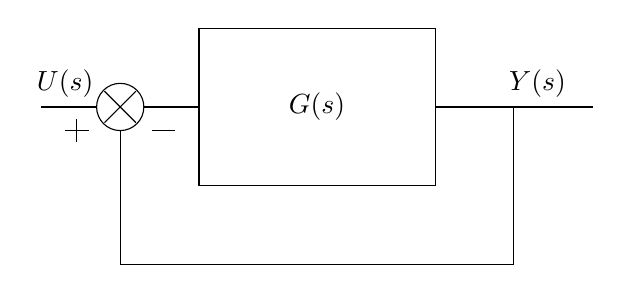
\begin{tikzpicture}
	\draw(0,0)--(7,0);
	\draw(1,0)--(1,-2)--(6,-2)--(6,0);
	\filldraw[draw=black, fill=white](2,-1)--(5,-1)--(5,1)--(2,1)--cycle;
	\draw[draw=black, fill=white] (1,0) circle (0.3);
	\draw(0.8,-0.2)--(1.2,0.2);
	\draw(0.8,0.2)--(1.2,-0.2);
	\draw(0.3,-0.3)--(0.6,-0.3);
	\draw(0.45,-0.15)--(0.45,-0.45);
	\draw(1.4,-0.3)--(1.7,-0.3);
	\node at (0.3,.3) {$U(s)$};
	\node at (6.3,.3) {$Y(s)$};
	\node at (3.5,0) {$G(s)$};
\end{tikzpicture}
\end{figure}

}\lineh
\\\\
$G(s)=\frac{s}{s^2+2s+1}$\\
$a_2=1 \ \ a_1 =2 \ \ a_0 = 1$\\
Układ zamknięty będzie asymptotycznie stabilny jeżeli układ otwarty będzie asymptotycznie stabilny oraz wykres charakterystyki amplitudowo-fazowej transformacji $G(s)$ nie będzie obejmował punktu (-1, 0) na płaszczyźnie zespolonej.\\
sprawdź czy układ otwarty jest asymptotycznie stabilny z Hurwitza. Wystarczy sprawdzić dla $s^2+2s+1$\\
$
\begin{array}{c}
\begin{array}{cc}a_1 & a_3\end{array}\\
\left[\begin{array}{cc}2&0\\1&1\end{array}\right]\\
\begin{array}{cc}a_0&a_2\end{array}
\end{array}
$\\
$2>0$\\
$2\cdot 1-0>0$\\
więc układ otwarty jest asymptotycznie stabilny.
$G(j\omega)=\frac{j\omega}{(j\omega)^2+2j\omega+1}=\frac{j\omega}{-\omega^2+2j\omega+1}=\frac{j\omega(1-\omega^2-2j\omega)}{(1-\omega^2+2j\omega)(1-\omega^2-2j\omega)}=\frac{j\omega-j\omega^3+2\omega^2}{1-2\omega^2+\omega^4+4\omega^2}=\frac{2\omega^2}{(\omega^2+1)^2}+j\frac{\omega-\omega^3}{(\omega^2+1)^2}$\\
\begin{figure}[!h]
\begin{tikzpicture}
	\draw[color=red, thick](1,0) ellipse (1 and 1);
	\filldraw[draw=white, fill=white](0,0)--(2,0)--(2,-2)--(0,-2)--cycle;
	\draw[color=red, draw opacity=0.1](1,0) ellipse (1 and 1);
	
	\draw[color=red!10!white] (1,-1) -- (1.2,-1.2);
	\draw[color=red!10!white] (1,-1) -- (1.2,-0.8);

	\draw[color=red] (1,1) -- (0.8,1.2);
	\draw[color=red] (1,1) -- (0.8,0.8);


	\draw[thick][->](-1,0)--(3,0) node [right=3pt]{$Re$};
	\draw[thick][->](0,-2)--(0,2) node [right=3pt]{$Im$};

	\node at(3.2,1){tylko górna część};

	\draw (-0.1,-1) -- (0.1,-1) node [left=2pt]{{-0.25}};
	\draw (-0.1,1) -- (0.1,1) node [left=2pt]{{0.25}};
	\draw (2,-0.1) -- (2,0.1) node [below=4pt]{{0.5}};
\end{tikzpicture}
\end{figure}
\noindent\\
Nie obejmuje punktu (-1,0) więc jest asymptotycznie stabilny.\\

%###################                 4.7.2              #################################%
%\pagebreak
%\subsection*{Zadanie 4.7.2} {\color{darkgray}
%	Niech będzie dany układ opisany transmitancją $G(s)$:\\
%	$G(s)=\frac{s^2+s+1}{s^3-s^2+2s-2}$\\
%	Korzystajac z kryterium Nyquista sprawdzić, czy układ zamkniety postaci 7 będzie asymptotycznie stabilny.
%\begin{figure}[!h]
%\begin{tikzpicture}
%	\draw(0,0)--(7,0);
%	\draw(1,0)--(1,-2)--(6,-2)--(6,0);
%	\filldraw[draw=black, fill=white](2,-1)--(5,-1)--(5,1)--(2,1)--cycle;
%	\draw[draw=black, fill=white] (1,0) circle (0.3);
%	\draw(0.8,-0.2)--(1.2,0.2);
%	\draw(0.8,0.2)--(1.2,-0.2);
%	\draw(0.3,-0.3)--(0.6,-0.3);
%	\draw(0.45,-0.15)--(0.45,-0.45);
%	\draw(1.4,-0.3)--(1.7,-0.3);
%	\node at (0.3,.3) {$U(s)$};
%	\node at (6.3,.3) {$Y(s)$};
%	\node at (3.5,0) {$G(s)$};
%\end{tikzpicture}
%\end{figure}
%
%}\lineh
%\\\\


%###################                 4.8.1              #################################%
\pagebreak
\subsection*{Zadanie 4.8.1} {\color{darkgray}
	Rozwiązanie równania różniczkowego\\
	$\dot{x}(t)=-4x(t)+3\sin(2t)$\\
	gdzie $x(0)=0, t \geqslant 0$ ma postać\\
	$x(t)=ae^{-4t}+A\sin(2t+\varphi)$\\
	Obliczyć $A$ i $\varphi$.\\
}\lineh
\\\\
$u(t)=3\sin(2t)$\\
$A_u=3 \ \ \ \ \omega = 2 \ \ \ \ \varphi_u=0$\\
$A=-4 \ \ \ B=3 \ \ \ \ C=1$\\
$G(s)=1\cdot(s+4)^{-1} \cdot 3=3 \cdot \frac{1}{s+4}$\\
$A(\omega)=|\frac{3}{2j+4}|=\frac{3}{\sqrt{16+4}}=\frac{3}{2\sqrt{5}}=\frac{3\sqrt{5}}{10}$\\
$A_y=3\cdot A(\omega)=\frac{9\sqrt{5}}{10}$\\
$\varphi_y=\arg G(j\omega)+\varphi_u$\\
$G(j\omega)=\frac{3}{2j+4}=\frac{3(4-2j)}{20}=\frac 3 5 -\frac{3}{10}j$\\
\fbox{\parbox{.24\linewidth}{
argument liczby $a+bi$ :\\
$\varphi=\begin{cases} \text{arctg}(\frac{b}{a}), a>0 \\ \text{arctg}(\frac ba)+\pi,a<0\end{cases}$
}}\\\\
$\arg G(j\omega)=\text{arctg}(-\frac{3}{10} \cdot \frac{5}{3})=\boxed{\text{arctg}(-\frac{1}{2})}$\\

%###################                 4.8.2              #################################%
%\pagebreak
%\subsection*{Zadanie 4.8.2} {\color{darkgray}
%	Rozwiązanie równania różniczkowego\\
%	$\dot{x}(t)=-x(t)+10\sin(5t+\frac\pi 3)$\\
%	gdzie $x(0)=0, t \geqslant 0$ ma postać\\
%	$x(t)=ae^{-4t}+A\sin(5t+\varphi)$\\
%	Obliczyć $A$ i $\varphi$.\\
%}\lineh
%\\\\

%###################                 4.9.1              #################################%
\pagebreak
\subsection*{Zadanie 4.9.1} {\color{darkgray}
	Rozwiązanie równania różniczkowego\\
	$\ddot{x}(t)+\dot{x}(t)=-4x(t)+3\sin({\omega t})$\\
	gdzie $x(0)=0$, ($\dot{x}(0)$ - w domysle), $t \geq 0$ ma postać\\
	$x(t)=f(t)+A\sin({\omega t+\varphi})$\\
	znaleźć takie $\omega$, dla którego $A$ jest największe\\
}\lineh
\\\\
$\ddot{x}(t)+\dot{x}(t)+4x(t)=3\sin({\omega t})$\\
$u(t)=\sin(\omega t)=\frac{\ddot{x}(t)+\dot{x}(t)+4x(t)}{3}$\\
$Y(s)=G(s)\cdot U(s) \Rightarrow G(s)=\frac{Y(s)}{U(s)}$\\
Transformata Laplace'a\\
$X(s)=Y(s)$\\
\fbox{\parbox{.3\linewidth}{
	$\mathcal{L}\{f'\}=s\mathcal{L}\{f\}-f(0^+)$\\
	$\mathcal{L}\{f''\}=s^2\mathcal{L}\{f\}-sf(0^+)-f'(0^+)$
}}\\\\
$U(s)=\frac{s^2X(s)-s\cdot x(0)-\dot{x}(0)+sX(s)-x(0)+4X(s)}{3}=\frac{X(s)(s^2+s+4)}{3}$\\
$G(s)=\frac{X(s)}{\frac{X(s)(s^2+s+4)}{3}}=\frac{3 \cancel{X(s)}}{ \cancel{X(s)}(s^2+s+4)}=\frac{3}{s^2+s+4}$\\
$A=\underbrace{A_y}_{\text{wyjście}}=\underbrace{A_u}_{\text{wejście}} \cdot A(\omega)$\\
$A(\omega)=|G(\omega j)|$\\
$A$ będzie maksymalne dla $|G(\omega j)|$ maksymalnego\\
$|G(\omega j)| = |\frac{3}{-\omega^2+j\omega+4}|=|\frac{3}{\sqrt{(4-\omega^2)^2+\omega^2}}|=|\frac{3}{\sqrt{16-8\omega^2+\omega^4+\omega^2}}|=|\frac{3}{\sqrt{\omega^4-7\omega^2+16}}|$\\
$\frac{3}{\sqrt{\omega^4-7\omega^2+16}}$ maksymalne $\Leftrightarrow \sqrt{\omega^4-7\omega^2+16}$ minimalne\\
$z=\omega^2$\\
szukamy min funkcji $z^2-7z+16$\\
dodatni znak przy $z^2$, więc minimum będzie na wierzchołku, czyli $x_w=\frac{-b}{2a}=\frac 72$\\
$\omega=\sqrt\frac 72 \ \ \ \vee \ \ \ \omega=-\sqrt\frac 72$\\
$\omega=-\sqrt\frac 72$ odpada, bo nie może być $<0$\\
$\boxed{\omega=\sqrt\frac 72}$\\





%###################                 4.9.2              #################################%
\pagebreak
\subsection*{Zadanie 4.9.2} {\color{darkgray}
	Rozwiązanie równania różniczkowego\\
	$\ddot{x}(t)+\dot{x}(t)=-x(t)+12\sin({\omega t})$\\
	gdzie $x(0)=0$, ($\dot{x}(0)$ - w domysle), $t \geq 0$ ma postać\\
	$x(t)=f(t)+A\sin({\omega t})$\\
	znaleźć takie $\omega$, dla którego $A$ jest największe\\
}\lineh
\\\\
$u(t)=\sin({\omega t})$\\
$y(t)=x(t)$\\\\
$\begin{cases} \ddot{x}(t)+\dot{x}(t)=-x(t)+12u(t)\\y(t)=x(t)\end{cases}$\\\\
$\left.\begin{cases} u(t)=\frac{\ddot{x}(t)+\dot{x}(t)+x(t)}{12}\\y(t)=x(t)\end{cases}\right|\mathscr{L}$\\\\
$\begin{cases} U(s)=\frac{s^2\cdot X(s)-s\cdot x(0)-\dot{x}(0)+sX(s)-x(0)+X(s)}{12}\\Y(s)=X(s)\end{cases}$\\\\
$\begin{cases} U(s)=\frac{s^2\cdot X(s)+sX(s)+X(s)}{12}\\Y(s)=X(s)\end{cases}$\\\\\\
$G(S)=\frac{Y(s)}{U(s)}=\frac{12\cdot \cancel{X(s)}}{\cancel{X(s)}\cdot (s^2+s+1)}=\frac{12}{s^2+s+1}$\\\\
$G(j\omega)=\frac{12}{-\omega^2+j\omega+1}=-\frac{12\cdot \omega^2-12}{\omega^4-\omega^2+1}-j\frac{12\cdot \omega}{\omega^4-\omega^2+1}$\\
$A_y=A_u\cdot ku(\omega)$\\
$ku(\omega)=|G(j\omega)|=\sqrt{\left(\frac{12\cdot \omega^2-12}{\omega^4-\omega^2+1}\right)^2+\left(\frac{12\cdot \omega}{\omega^4-\omega^2+1}\right)^2}=12\cdot \sqrt{\frac{1}{\omega^4-\omega^2+1}}$\\\\\\
$A_y$ będzie max., gdy $ku(\omega)$ będzie max., tj. $\sqrt{\omega^4-\omega^2+1}$ będzie min.
$\omega \geq 0$, $min(\sqrt{\omega^4-\omega^2+1})$ dla $\omega=\frac{1}{\sqrt{2}}$


%###################                 4.9.3              #################################%
%\pagebreak
%\subsection*{Zadanie 4.9.3} {\color{darkgray}
%	Rozwiązanie równania różniczkowego\\
%	$\ddot{x}(t)+\dot{x}(t)=-5x(t)+15\sin({\omega t})$\\
%	gdzie $x(0)=0$, ($\dot{x}(0)$ - w domysle), $t \geq 0$ ma postać\\
%	$x(t)=f(t)+A\sin({\omega t+\varphi})$\\
%	znaleźć takie $\omega$, dla którego $A$ jest największe\\
%}\lineh
%\\\\

%###################                 4.10.1              #################################%
\pagebreak
\subsection*{Zadanie 4.10.1} {\color{darkgray}
	Korzystając z kryterium Michajłowa zbadać stabilność asymptotyczną układu opisanego transmitancją $G(s)$:\\
	$G(s)=\frac{s^2+3s+1}{s^3+s^2-4s+9}$\\
}\lineh
\\\\
\fbox{\parbox{.6\linewidth}{
	\textbf{Kryterium Michajłowa}\\
	$G(s)=\frac{L(s)}{M(s)}$\\
	$M(s)=a_ns^n+a_{n-1}s^{n-1}+...+a_1s+a_0$\\
	Układ jest asymptotycznie stabilny jeśli przyrost argumentu $M(j\omega)$ rzędu $n$ przy zmianie $\omega$ od $-\infty$ do $+\infty$ wynosi $n\pi$: $\Delta Arg \ M(j\omega)|^{+\infty}_{-\infty}=n\pi$\\
}}\\\\
Ponieważ funkcja $M(j\omega)$ jest symetryczna względem osi rzeczywistej, więc wystarczy $\Delta Arg \ M(j\omega)|^{+\infty}_0=n\frac\pi 2$\\
inna postać kryterium (wynikająca z powyższego):
wystarczy pokazać, że charakterystyka częstotliwościowa funkcji $M(j\omega) \ \ 0<\omega <\infty$ przechodzi przez $n$ ćwiartek w kierunku dodatnim.\\
$n=3$ więc musi przechodzić przez I, II i III ćwiartkę\\
$M(s)=s^3+s^2-4s+9$\\
$M(j\omega)=-j\omega^3-\omega^2-4j\omega+9=\underbrace{9-\omega^2}_{Re}+j\underbrace{(-\omega^3-4\omega)}_{Im}$\\
$\omega=0 \Rightarrow M(j0)=9$\\
\begin{figure}[!h]
\begin{tikzpicture}
	\draw [color=red, thick](2,0) arc (0:90:2 and 1.5);
	\draw [color=red, thick](0,1.5) arc (90:180:1 and 1.5);
	\draw [color=red, thick](-1,0) arc (180:220:1.5 and 3);

	\draw[thick][->](-3,0)--(3,0) node [right=3pt]{$Re$};
	\draw[thick][->](0,-3)--(0,3) node [right=3pt]{$Im$};

	\draw (1.3,1.2) -- (2,1.2);
	\draw (1.3,1.2) -- (1.5,1.3);
	\draw (1.3,1.2) -- (1.5,1.1);

	\node at(4.2,1.2){powinny być tak, żeby był a.s.};


	\draw (-0.1,-2) -- (0.1,-2) node [left=3pt]{{-39}};
	\draw (2,-0.1) -- (2,0.1) node [below=4pt]{{9}};
\end{tikzpicture}
\end{figure}
\noindent\\
spr. gdzie przecina $Im$ dla $Re=0$\\
$9-\omega^2=0\Rightarrow\omega=3$\\
$Im=-3^3-4\cdot 3=-39$ {\color{lightgray} ($Im$ powinno być dodatnie, aby układ był asymptotycznie stabilny)}\\
spr. czy przecina oś $Re$ w przedziale $(-\infty, 0)$\\
$Im=0\Rightarrow -\omega(\omega^2+4)=0$\\
$\omega=0 \ \ \ \omega^2=-4$\\
$Re=9+4=13$\\
więc, układ nie jest asymptotycznie stabilny.

%###################                 4.12.1              #################################%
\subsection*{Zadanie 4.12.1}
Dla filtru dolnoprzepustowego typu RC dobrać tak wartość kondensatora i opornika by przy częstotliwości $10^-2 Hz$ wzmocnienie wynosiło 0 dB

\begin{figure}[h!]
\centering
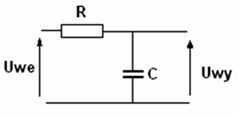
\includegraphics[width=0.4\linewidth]{RCdiagram4_12_1}
\caption{Filtr dolnoprzepustowy}
\label{fig:RCdiagram4}
\end{figure}
Dla układu jak na rysunku (\ref{fig:RCdiagram4}) wyznaczam transmitancję:

\begin{equation}
\left\lbrace \begin{array}{rcl}
u_{we} - u_R - u_{wy} &=& 0 \\
u_{R} &=& i  R \\
i &=& C  \frac{d u_{wy}}{dt} \\
\end{array}\right.
\end{equation}
 




\begin{align} 
u_{we} - RC \frac{d u_{wy}}{dt} - u_{wy} &= 0 \\
 \frac{d u_{wy}}{dt} + \frac{1}{RC}  u_{wy} &= \frac{1}{RC} u_{we}    \quad /\ \mathcal{L} \\
 s U_{wy} + \frac{1}{RC}  U_{wy} &= \frac{1}{RC} U_{we} \\
 U_{wy}  \left(  s+ \frac{1}{RC}\right) &=  \frac{1}{RC} U_{we} \\
\end{align}
w takim razie:
\begin{align} 
G(s)  = \frac{U_{wy}}{U_{we}} &= \frac{\frac{1}{RC}}{s+ \frac{1}{RC} }\\
 G(s) &= \frac{1}{1 + sRC} \\
\end{align}
Wzmocnienie to:




\begin{equation}
\frac{u_{wy}(t)}{u_{we}(t)} = |G(j\omega)| = \left| \frac{1}{1 + sRC} \right|  = \frac{1}{\sqrt{1 + \omega^2 R^2 C^2}}
\end{equation}

Wzmocnienie w decybelach:
\begin{align}
k = 20\log\left( \frac{u_{wy}}{u_{we}}\right)  &= 0 \; dB  \longleftarrow \text{ \it{jak inne wzmocnienie to tutaj wstawić}} \\
\log\left( \frac{u_{wy}}{u_{we}}\right)  &= 0  = \log(1)  \Longrightarrow \frac{u_{wy}}{u_{we}} = 1 \\
\end{align}
a zatem:
\begin{equation}
\frac{1}{\sqrt{1 + \omega^2 R^2 C^2}} = 1 \Longrightarrow \omega^2 R^2 C^2 = 0 \label{eq:wRC=0}
\end{equation}
Z założenia zadania:
\begin{align}
\omega &= 2\pi f \\
\omega &= 2 \pi \cdot 10^{-2} \left[ \frac{1}{s} \right] \longleftarrow \text{ \it{jak inna częstotliwość to tutaj wstawić}} \label{eq:w=2pi*f} \\
\end{align}

Z (\ref{eq:wRC=0}) i (\ref{eq:w=2pi*f}) wynika, że:
\begin{equation}
RC = 0 \quad \Longrightarrow \quad R=0 \vee C=0
\end{equation}
Wystarczy przyjąć, że $R = 0$ i $C$ jest dowolne

%###################                 4.13.1              #################################%

\subsection*{Zadanie 4.13.1}
Obliczyć przesunięcie fazowe przy pulsacji $0.5 \frac{rad}{s}$dla członu całkującego przy wzmocnieniu $-0.5 e$

\vspace{1em}

Człon całkujący daje na wyjściu sygnał $x(t)$ proporcjonalny do całki sygnału wejściowego $u(t)$.
\begin{align}
x(t) &= k \int_{0}^{t} u(\tau) \; d\tau \Longleftrightarrow X(s) = k \frac{1}{s} U(s) \\
G(s) &= \frac{k}{s} \\
k &= -\frac{e}{2} \Leftarrow \text{wynika z treści zadania} \\
 \label{eq:G(s)}G(s) &=  - \frac{e}{2s}
\end{align} 

Wiadomo, że układ  transmitancji $G(s)$ wprowadza przesunięcie fazowe:
\begin{equation}
\label{eq:phi}
\phi = \arg G(j\omega)
\end{equation}

Pulsacja układu na podstawie treści zadania wynosi:
\begin{equation}
\label{eq:omega}
 \omega = 0.5 \frac{rad}{s}
\end{equation}
Na podstawie (\ref{eq:G(s)}) ,  (\ref{eq:phi}) i  (\ref{eq:omega}):
\begin{equation}
\begin{split}
\phi = \arg G\left( \frac{1}{2} j\right)  = \arg \left( - \frac{e}{ 2 \cdot \frac{1}{2} j}  \right)   = \arg \left( - \frac{e}{j} \right) =  \\ \arg \left( - \frac{e}{j}\cdot \frac{j}{j} \right)  = \arg \left( - \frac{e j}{-1} \right) = \arg \left( e j \right) 
\end{split}
\end{equation}
Dla przypomnienia funkcja $\arg()$ to argument liczby zespolonej, czyli $ \arctan\left( \frac{b}{a}\right) $, gdzie $a$ to część rzeczywista, a $b$ to część zespolona.

W naszym przypadku mamy tylko cześć urojoną, a więc stosunek $ \frac{b}{a}$ jest równy $\infty$ 
\begin{equation}
\phi = \arg(ej) = \arctan(\infty) = \frac{\pi}{2}
\end{equation}


%`x(t) = k * całka (od 0 do t) u(tau) d(tau) <=> X(s) = k/s*U(s)
%G(s) = k/s
%W zadaniu k = -0.5 e = -e/2
%Wiadomo, że układ  transmitancji G(s) wprowadza przesunięcie fazowe fi = arg G(jw)
%Pulsacja układu to omega = 0.5 rad / s
%czyli fi = arg G(j * ½) = arg [ (-e/2)  / (j*1/2) ]  = arg (j*e/1) = arg (j*e) = pi/2
%Przesunięcie fazowe wprowadzane przez człon całkujący wynosi zatem pi/2


%###################                 4.10.2              #################################%
%\pagebreak
%\subsection*{Zadanie 4.10.2} {\color{darkgray}
%	Korzystając z kryterium Michajłowa zbadać stabilność asymptotyczną układu opisanego transmitancją $G(s)$:\\
%	$G(s)=\frac{s^2+s+1}{s^3-s^2+2s-2}$\\
%}\lineh
%\\\\

%  \left[\begin{array}{cc}\end{array}\right]